\subsection{Speisung}
\label{subsec:Speisung}
Um die Speisung des Analog- bzw. des Digital-Teils zu verifizieren wurde die Spannung nach den jeweiligen LDOs mit einem Agilent 34410A Multimeter gemessen. Die USB-Versorgungs-Spannung schwankt je nach Quelle zwischen 4.9 und 5.2V, jedoch sollte sie nach den LDOs konstant 3.3V betragen. Gemessen wurden folgende Spannungen:

\textbf{Spannung am Analog-LDO:} 3.2924V\\
\textbf{Spannung am Digital-LDO:} 3.2957V

Weiter wurden die Spitzen der Spannungsversorgung mit einem Tektronix TDS 2014C Oszilloskop gemessen. Als Vergleich einmal vom Stromnetz und einmal von einer handelsüblichen Powerbank gespiesen.

\begin{figure} [H]
\begin{minipage}[c]{0.5\textwidth}
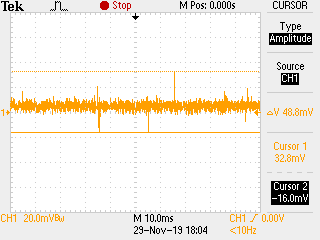
\includegraphics[width=\textwidth]{graphics/Speisung_Netz_Analog.png}
\end{minipage}
\begin{minipage}[c]{0.5\textwidth}
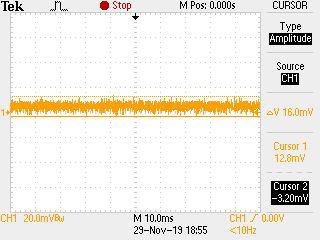
\includegraphics[width=\textwidth]{graphics/Speisung_PB_Analog.png}
\end{minipage}
\caption{Vergleich der analogen Speisung am Netz (links) und mit einer Powerbank (rechts)}
\label{fig:analogspeisung}
\end{figure} 

\begin{figure} [H]
\begin{minipage}[c]{0.5\textwidth}
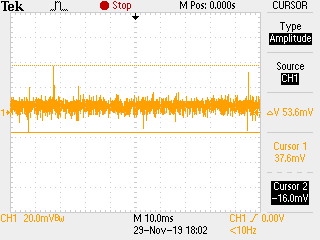
\includegraphics[width=\textwidth]{graphics/Speisung_Netz_Digital.png}
\end{minipage}
\begin{minipage}[c]{0.5\textwidth}
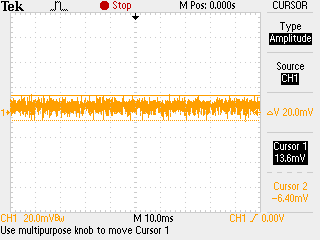
\includegraphics[width=\textwidth]{graphics/Speisung_PB_Digital.png}
\end{minipage}
\caption{Vergleich der digitalen Speisung am Netz (links) und mit einer Powerbank (rechts)}
\label{fig:digitalspeisung}
\end{figure} 

Wie in Abbildungen \ref{fig:analogspeisung} und \ref{fig:digitalspeisung} ersichtlich macht die unterschiedliche Speisung vom Netz sowie der Powerbank einen Unterschied in den Spannungsspitzen. Die Spitzen erreichen 50mV Peak-Peak, was jedoch von den Stützkondensatoren am Microcontroller und am Codec geglättet wird. Das Grundrauschen der Spannung von 20mV ist vertretbar. Die Speisung funktioniert wie erwartet.